\section{Modul Semisederhana}
Bagian ini menggunakan konvensi praktis berikut, yang merupakan kasus khusus Konvensi \ref{con:Hom-assoc}.
\begin{convention}\label{con:left-right-End}
	Misalkan $M$ adalah modul kiri $R$ tak nol dan definisikan gelanggang $A := \End_R(M)^\text{op}$. Maka $M$ secara natural menjadi modul kanan $A$ melalui perkalian kanan berikut:
	\[ (m, a) \mapsto a(m), \quad m \in M, \; a \in A;  \]
Gelanggang lawan dari $\End_R(M)$ diambil untuk menyesuaikan penulisan lazim bagi komposisi peta. Sesungguhnya $M$ dengan demikian merupakan bimodul-$(R,A)$: hukum asosiatif $r(ma) = (rm)a$ mencerminkan linearitas-$R$ dari peta $a$.

	Demikian pula, untuk modul kanan $R$ tak nol $M$, tetapkan $A := \End_R(M)$. Perkalian kiri $(a, m) \mapsto a(m)$ memberi $M$ struktur bimodul-$(A,R)$ yang natural, dan tetap berlaku hukum asosiatif $a(mr) = (am)r$.
\end{convention}

Kembali ke pokok bahasan. Konsep modul sederhana telah disebutkan dalam Definisi \ref{def:submodule}; sekarang kita mengkajinya lebih lanjut. Kecuali dinyatakan lain, bagian ini terutama meninjau modul kiri atas gelanggang $R$. Beberapa contoh:
\begin{itemize}
	\item Misalkan $\mathfrak{a} \subset R$ adalah ideal kiri. Hasil bagi $R/\mathfrak{a}$ sederhana jika dan hanya jika $\mathfrak{a}$ merupakan ideal kiri maksimal.
	\item Ruang vektor $V$ atas gelanggang pembagian $D$ merupakan modul $D$ sederhana jika dan hanya jika $\dim_D V = 1$.
	\item Misalkan $D$ adalah gelanggang pembagian, $V$ ruang vektor kanan $D$ tak nol, dan definisikan gelanggang $R := \End(V_D)$. Beri $V$ struktur modul kiri $R$ menurut Konvensi \ref{con:left-right-End}. Karena setiap $v \in V \smallsetminus \{0\}$ memenuhi $Rv = V$, maka $V$ selalu sederhana sebagai modul $R$. Kasus konkret yang lazim ialah menetapkan $n \in \Z_{\geq 1}$ dan memandang $V = D^n$ sebagai vektor kolom (vertikal); dalam hal ini $R$ dapat diidentifikasi dengan gelanggang matriks $M_n(D)$ yang bekerja pada $V$ melalui perkalian matriks dari kiri.

	Jika yang ditinjau adalah ruang vektor kiri $D$, maka $V$ harus dipandang sebagai modul kanan $R^\text{op}$. Ketika $V = D^n$ dipandang sebagai vektor baris (horizontal), interpretasi matriks di atas tetap berlaku dengan perkalian kanan menggantikan perkalian kiri.
\end{itemize}

\begin{lemma}[Lemma Schur]\label{prop:Schur-mod}\index{Lemma Schur}
	Misalkan $M_1$ dan $M_2$ adalah modul sederhana. Setiap $\varphi \in \Hom_R(M_1, M_2)$ merupakan isomorfisme atau homomorfisme nol. Khususnya, untuk setiap modul sederhana $M$, gelanggang endomorfisme $\End_R(M)$ merupakan gelanggang pembagian.
\end{lemma}
\begin{proof}
	Modul sederhana tak nol menurut definisi. Dengan menggunakan kesederhanaannya, berlaku salah satu dari dua kemungkinan: $\Ker(\varphi) = M_1$, sehingga $\varphi=0$; atau $\Ker(\varphi)=0$, sehingga $M_1 \simeq \Image(\varphi) = M_2$ dan $\varphi$ merupakan isomorfisme.
\end{proof}

Sebagai akibat, misalkan diberikan dekomposisi jumlah langsung hingga $M = \bigoplus_{i=1}^r M_i^{\oplus n_i}$, dengan $M_1, \ldots, M_r$ modul-modul sederhana yang saling tak isomorfik. Lemma \ref{prop:Hom-matrix} memberikan
\[ \End_R(M)^{\text{op}} \rightiso \prod_{i=1}^n M_{n_i}\left(D_i^{\text{op}}\right)^{\text{op}} \xrightarrow[\text{transpos}]{\sim} \prod_{i=1}^n M_{n_i}(D_i) \]
dengan $D_i := \End_R(M_i)^\text{op}$ suatu gelanggang pembagian, $M_i^{\oplus n_i}$ suatu modul kanan $M_{n_i}(D_i)$, dan $M$ suatu modul kanan $\End_R(M)^\text{op}$; isomorfisme di atas mempertahankan struktur-struktur modul tersebut.

\begin{lemma}\label{prop:existence-simple-subquotient}
	Untuk setiap modul tak nol $M$, terdapat submodul $M_2 \subset M_1 \subset M$ sedemikian sehingga $M_1/M_2$ sederhana.
\end{lemma}
\begin{proof}
	Pilih $m \in M \smallsetminus \{0\}$, tetapkan $M_1 := Rm$, dan definisikan ideal kiri $R$, $\mathfrak{a} := \Ker[R \xrightarrow{r \mapsto rm} M_1]$, sehingga $R/\mathfrak{a} \simeq M_1$. Menurut Lemma Zorn (Teorema \ref{prop:Zorn}), terdapat ideal kiri maksimal $\mathfrak{b} \supset \mathfrak{a}$. Ambil submodul $M_2 \subset M_1$ yang bersesuaian dengan $\mathfrak{b}/\mathfrak{a} \subset R/\mathfrak{a}$.
\end{proof}

\begin{proposition}\index{mo!semisederhana (semisimple)}
	Untuk modul $M$, syarat-syarat berikut ekuivalen:
	\begin{enumerate}[(i)]
		\item $M$ dapat dinyatakan sebagai jumlah suatu keluarga submodul sederhana: $M = \sum_{i \in I} M_i$.
		\item $M$ dapat dinyatakan sebagai jumlah langsung suatu keluarga submodul sederhana: $M = \bigoplus_{i \in I} M_i$.
		\item Setiap submodul $M' \subset M$ merupakan suku langsung; dengan kata lain, terdapat submodul $M'' \subset M$ sedemikian sehingga $M = M' \oplus M''$.
	\end{enumerate}
	Modul $M$ yang memenuhi syarat-syarat ekuivalen di atas disebut \emph{modul semisederhana}.
	
	Dalam barisan eksak pendek $0 \to M' \to M \to M'' \to 0$, jika $M$ semisederhana, maka $M'$ dan $M''$ juga semisederhana.
\end{proposition}
\begin{proof}
	Pertama, buktikan bahwa jika syarat (iii) berlaku untuk $M$ dalam suatu barisan eksak pendek $0 \to M' \to M \to M'' \to 0$, maka syarat tersebut juga berlaku untuk $M'$ dan $M''$. Misalkan $M'_0 \subset M'$ adalah submodul. Menurut asumsi, terdapat $N \subset M$ sehingga $M = M'_0 \oplus N$. Mudah diperiksa bahwa $M' = M'_0 \oplus (N \cap M')$, sehingga (iii) berlaku untuk $M'$. Di sisi lain, menurut asumsi $M'$ merupakan suku langsung: $M \simeq M' \oplus S$. Maka $M'' \simeq M/M'$ isomorfik dengan submodul $S$ dari $M$, sehingga langkah sebelumnya menunjukkan bahwa $M''$ juga memenuhi (iii). Ini sekaligus membuktikan bagian terakhir proposisi.

	Sekarang buktikan (i) $\implies$ (ii). Misalkan $M = \sum_{i \in I} M_i$, dengan setiap $M_i$ submodul sederhana. Tetapkan
	\[ \mathcal{J} := \left\{ J \subset I: \sum_{i \in J} M_i \;\text{merupakan jumlah langsung} \right\}. \]
Kita akan menggunakan Lemma Zorn untuk membuktikan bahwa himpunan terurut parsial $(\mathcal{J}, \subset)$ mempunyai unsur maksimal. Karena jumlah kosong didefinisikan sebagai modul nol, $\emptyset \in \mathcal{J}$ dan $\mathcal{J} \neq \emptyset$. Kami menyatakan bahwa setiap rantai dalam $(\mathcal{J}, \subset)$ mempunyai batas atas. Memang, untuk subhimpunan terurut total $\mathcal{J}' \subset \mathcal{J}$, gabungan $J' := \cup_{J \in\mathcal{J}'} J$ tetap termasuk $\mathcal{J}$, sebab $\sum_{i \in J'} M_i$ merupakan jumlah langsung jika dan hanya jika
	\[ \forall i \in J', \; M_i \cap \sum_{\substack{j \in J' \\ j \neq i}} M_j = \{0\}, \]
dan syarat ini cukup diperiksa pada setiap subhimpunan hingga dari $J'$.
	
	Ambil $J$ sebagai unsur maksimal $(\mathcal{J}, \subset)$. Jika $\bigoplus_{i \in J} M_i = M$, diperoleh (ii). Jika tidak, terdapat $k \in I$ sehingga $M_k \not\subset \bigoplus_{i \in J} M_i$. Karena $M_k$ sederhana, $M_k \cap \bigoplus_{i \in J} M_i = \{0\}$, dan ini mengakibatkan $J \sqcup \{k\} \in \mathcal{J}$, suatu kontradiksi.
	
	Sekarang buktikan (ii) $\implies$ (iii). Ambil sebarang submodul $M' \subset M = \bigoplus_{i \in I} M_i$ dan tetapkan
	\[ \mathcal{J} := \left\{ J \subset I: M' + \bigoplus_{i \in J} M_i \; \text{merupakan jumlah langsung} \right\}. \]
Dengan meniru argumen sebelumnya, diperoleh unsur maksimal $J \in \mathcal{J}$. Kami menyatakan bahwa $M'' := \bigoplus_{i \in J} M_i$ memenuhi $M = M' \oplus M''$. Jika tidak, terdapat $k \in I$ sehingga $M_k \not\subset M' \oplus M''$. Kesederhanaan mengakibatkan $M_k \cap (M' \oplus M'') = \{0\}$, sehingga $J \sqcup \{k\} \in \mathcal{J}$, suatu kontradiksi.
	
	Sekarang buktikan (iii) $\implies$ (i). Kami menyatakan bahwa setiap submodul tak nol $M' \subset M$ mempunyai submodul sederhana. Andaikan sifat ini dan definisikan $\text{soc}(M)$ sebagai jumlah semua submodul sederhana dalam $M$. Menurut (iii), terdapat $M' \subset M$ sehingga $M = \text{soc}(M) \oplus M'$. Jika $M' \neq \{0\}$, terdapat submodul sederhana $N \subset M'$, dan $N \subset \text{soc}(M) \cap M' = \{0\}$ memberikan kontradiksi.

	Pernyataan terakhir dibuktikan sebagai berikut. Lemma \ref{prop:existence-simple-subquotient} memberikan subkuosien sederhana $M_1/M_2$ dari $M'$. Awal pembuktian telah menunjukkan bahwa $M'$ dan $M_1$ mewarisi sifat (iii) dari $M$. Maka terdapat penanaman $M_1/M_2 \hookrightarrow M_1 \subset M'$, yang memberikan submodul sederhana yang dicari.
\end{proof}

Pembuktian di atas memperkenalkan konsep \emph{sokel} bagi sebarang modul $M$, yang didefinisikan sebagai
\[ \text{soc}(M) := \sum_{\substack{N \subset M \\ \text{submodul sederhana} }} N, \]
dengan kata lain, $\text{soc}(M)$ adalah submodul semisederhana maksimal dari $M$. Bayangan homomorfik suatu modul sederhana adalah nol atau tetap sederhana. Karena itu, setiap homomorfisme modul $\varphi: M_1 \to M_2$ menginduksi $\text{soc}(\varphi): \text{soc}(M_1) \to \text{soc}(M_2)$. Dengan kata lain, $\text{soc}(-)$ mendefinisikan fungtor dari $R\dcate{Mod}$ ke subkategori penuh $R\dcate{Mod}_{\text{ss}}$ yang terdiri atas modul-modul semisederhana.

Konsep lain yang berguna ialah \emph{semisimplifikasi} modul berpanjang hingga $M$: tetapkan
\[ M_\text{ss} := \bigoplus_{N \in \text{JH}(M)} N, \]
dengan multiplisitas faktor Jordan--Hölder diperhitungkan dalam jumlah langsung. Walaupun kelas isomorfisme $M_\text{ss}$ ditentukan secara tunggal oleh Teorema \ref{prop:JH-mod}, pemetaan $M \mapsto M_\text{ss}$ bukanlah fungtor, sebab definisinya melibatkan pemilihan deret komposisi.

Lemma Fitting berikut secara mengejutkan berguna dalam banyak masalah matematika; kita akan menggunakannya dalam \S\ref{sec:indecomposable-mod}.
\begin{lemma}[H.\ Fitting]\label{prop:Fitting}
	Misalkan $M$ adalah modul tak nol berpanjang hingga dan $u \in \End_R(M)$. Terdapat dekomposisi kanonik
	\[ M = \Ker(u^\infty) \oplus \Image(u^\infty) \]
dengan $\Ker(u^\infty)$ dan $\Image(u^\infty)$ invarian di bawah aksi $u$, serta
	\begin{compactitem}
		\item $u|\Image(u^\infty)$ merupakan automorfisme invertibel dari $\Image(u^\infty)$,
		\item $u|\Ker(u^\infty)$ merupakan endomorfisme nilpoten dari $\Ker(u^\infty)$.
	\end{compactitem}
\end{lemma}
\begin{proof}
	Karena $M$ berpanjang hingga, rantai submodul
	\begin{gather*}
		\Ker(u) \subset \Ker(u^2) \subset \cdots, \\
		\Image(u) \supset \Image(u^2) \supset \cdots
	\end{gather*}
masing-masing berhenti pada $\Ker(u^\infty)$ dan $\Image(u^\infty)$; mudah dilihat bahwa keduanya invarian-$u$. Tugas utama ialah membuktikan dekomposisi jumlah langsung $M = \Ker(u^\infty) \oplus \Image(u^\infty)$. Pilih $n \gg 0$ sehingga $\Ker(u^\infty) = \Ker(u^n)$ dan $\Image(u^\infty) = \Image(u^n)$. Jika $x \in \Image(u^\infty)$, $x = u^n(y_n)$, memenuhi $u^n(x)=0$, maka $y_n \in \Ker(u^{2n})=\Ker(u^n)$, sehingga $x=0$. Jadi $\Ker(u^\infty) \cap \Image(u^\infty) = \{0\}$.
	
	Di sisi lain, setiap $x \in M$ dapat dinyatakan sebagai
	\[ x = (\underbracket{x - u^n(y)}_{\in \Ker(u^n)}) + \underbracket{u^n(y)}_{\in \Image(u^n)}, \qquad y \in M, \; u^n(x) = u^{2n}(y), \]
keberadaan $y$ demikian mengikuti dari $\Image(u^n) = \Image(u^{2n})$. Maka $\Ker(u^\infty) + \Image(u^\infty) = M$, sehingga dekomposisi jumlah langsung terbukti.

Mudah dilihat bahwa $u|\Ker(u^\infty)$ nilpoten dan $u|\Image(u^\infty)$ surjektif. Dari $\Ker(u) \cap \Image(u^\infty) \subset \Ker(u^\infty) \cap \Image(u^\infty) = \{0\}$, diperoleh bahwa $u|\Image(u^\infty)$ juga injektif. Selesai.
\end{proof}

\section{Modul Tak Terurai}\label{sec:indecomposable-mod}
Sebelum mengkaji modul tak terurai lebih jauh, terlebih dahulu kita tinjau konsep yang sedikit lebih umum. Ingat kembali Definisi \ref{def:additive-cat} tentang kategori aditif.

\begin{definition}\index{duixiang!tak terurai (indecomposable)}
	Objek tak nol $M$ dalam kategori aditif $\mathcal{C}$ disebut \emph{tak terurai} jika ia hanya mempunyai satu ekspresi biproduk $M = X \oplus Y$ (lihat Definisi \ref{def:biproduct} beserta notasinya, dengan mengabaikan urutan), yaitu yang diberikan oleh $\iota_1 = p_1: M \xrightarrow{\identity} M$ dan morfisme nol $\begin{tikzcd} 0 \arrow[yshift=0.6ex, r, "\iota_2"] & M \arrow[yshift=-0.6ex, l, "p_2"] \end{tikzcd}$; dengan kata lain, biproduk trivial $X=M$, $Y=0$.
\end{definition}

Tetapkan suatu gelanggang $R$. Penerapan definisi tersebut pada kategori aditif $R\dcate{Mod}$ memberikan konsep \emph{modul tak terurai}. Sifat ini umumnya lebih lemah daripada kesederhanaan. \index{mo!tak terurai (indecomposable)}
\begin{example}
	Misalkan $R$ adalah daerah ideal utama, $\mathfrak{p}$ suatu ideal prima tak nol di dalamnya, dan $n \geq 1$. Maka modul $R$, $R/\mathfrak{p}^n$, tak terurai, tetapi tidak sederhana jika $n \geq 2$.
\end{example}

Himpunan endomorfisme dalam kategori aditif memiliki struktur gelanggang. Suatu unsur $a$ dalam gelanggang disebut \emph{idempoten} jika $a^2=a$, dan disebut \emph{nilpoten} jika terdapat $m > 1$ sehingga $a^m=0$. Bagian ini juga memerlukan konsep berikut.\index{nilpoten (nilpotent)} \index{idempoten (idempotent)}
\begin{definition}\label{def:noncommutative-local-ring}\index{huan!lokal (local)}
	Dalam bagian ini, suatu gelanggang $S$ disebut gelanggang lokal jika subhimpunan $S \smallsetminus S^\times$ merupakan ideal dua sisi.
\end{definition}
Jika $S$ komutatif, syarat ini ekuivalen dengan $S$ mempunyai ideal maksimal tunggal $\mathfrak{m} := S \smallsetminus S^\times$, yakni definisi lazim gelanggang komutatif lokal.

Pertama, tinjau dekomposisi jumlah langsung berhingga $M = \bigoplus_{i=1}^n M_i$ dari suatu objek tak nol dalam kategori aditif $\mathcal{C}$. Menurut kasus $n$-ary dari Definisi \ref{def:biproduct} tentang biproduk, untuk setiap $1 \leq i \leq n$ terdapat morfisme proyeksi
\begin{align*}
	p_i: M & \twoheadrightarrow M_i \\
	\sum_{j=1}^n m_j & \mapsto m_i, \quad \forall j, \; m_j \in M_j,
\end{align*}
yang, setelah dikomposisikan dengan morfisme inklusi $\iota_i: M_i \hookrightarrow M$, memberikan $e_i = \iota_i p_i \in \End(M)$. Unsur-unsur ini mempunyai sifat-sifat berikut:
\begin{enumerate}[\bfseries {E}.1]
	\item $e_i$ idempoten: $e_i^2 = (\iota_i p_i) (\iota_i p_i) = \iota_i (p_i \iota_i) p_i = \iota_i p_i$.
	\item Ortogonalitas: $i \neq j \implies e_i e_j = \iota_i p_i \iota_j p_j = 0$.
	\item Persamaan $\sum_{i=1}^n e_i = 1$ berlaku dalam gelanggang $\End(M)$.
\end{enumerate}
Perhatikan bahwa $e_i = 1 \iff M_i = M$, sedangkan $e_i = 0 \iff M_i = \{0\}$.

Selanjutnya tetapkan gelanggang $R$ dan tinjau kasus kategori $\mathcal{C} = R\dcate{Mod}$. Dalam hal ini, suku langsung $M_i$ dapat dikarakterisasi oleh kernel morfisme idempoten: $\iota: M_i \rightiso \Ker(\sum_{j \neq i} e_j) \subset M$. Sebaliknya, diberikan suatu keluarga unsur idempoten $(e_i)_{i=1}^n$ yang memenuhi \textbf{E.1} --- \textbf{E.3}, definisikan kernel $M_i := \Ker(\sum_{j \neq i} e_j) \xrightarrow{\iota_i} M$ seperti di atas. Jelas bahwa $\Image(e_i) \subset M_i$, sehingga $e_i$ dapat difaktorkan sebagai $\iota_i p_i$, dengan $p_i: M \to M_i$. Kita memperoleh
\begin{align*}
	\forall i,j, \; p_i \iota_j & = \begin{cases}
		\identity_{M_i}, & i=j \\
		0, & i \neq j
	\end{cases} \quad \because\text{diperiksa setelah mengomposisikan kedua ruas dengan monomorfisme $\iota_i$ dari kiri}, \\
	\sum_{i=1}^n \iota_i p_i & = \sum_{i=1}^n e_i = \identity_M.
\end{align*}
Ini tepat merupakan versi $n$-ary dari Definisi \ref{def:biproduct} tentang biproduk, sehingga $\bigoplus_{i=1}^n M_i = M$.

\begin{proposition}\label{prop:direct-sum-idempotent}
	Untuk setiap objek tak nol $M$ dari $R\dcate{Mod}$, cara di atas memberikan bijeksi
	\[\begin{tikzcd}
		\left\{ \text{dekomposisi jumlah langsung} M = \bigoplus_{i=1}^n M_i, \; M_i \subset M \right\} \arrow[leftrightarrow, d, "1:1"] \\
		\left\{ \End_R(M)\; \text{dengan keluarga idempoten}\; (e_i)_{i=1}^n : \text{memenuhi sifat \textbf{E.1} --- \textbf{E.3}} \right\},
	\end{tikzcd}\]
Penataan ulang suku-suku dekomposisi jumlah langsung bersesuaian dengan penataan ulang $e_1, \ldots, e_n$. Modul $M$ tak terurai jika dan hanya jika dalam gelanggang $\End_R(M)$ berlaku $e^2 = e \implies (e=0 \vee e=1)$.
\end{proposition}
\begin{proof}
	Mudah dilihat bahwa kedua pemetaan di atas (dekomposisi jumlah langsung $\leftrightarrow$ keluarga idempoten) saling invers dan jelas mempertahankan aksi penataan ulang. Jika $n=2$, pembahasan di atas menunjukkan bahwa dekomposisi jumlah langsung $M = X \oplus Y$ berkorespondensi bijektif dengan unsur idempoten $e \in \End_R(M)$; dekomposisi trivial bersesuaian dengan $e = 0,1$.
\end{proof}
Diberikan suatu keluarga unsur idempoten $(e_i)_{i=1}^n$ yang memenuhi \textbf{E.1} dan \textbf{E.2}, tambahkan unsur idempoten $e_{n+1} := 1 - \sum_{i=1}^n e_i$. Keluarga yang diperluas, $(e_i)_{i=1}^{n+1}$, tetap ortogonal dan memenuhi $\sum_{i=1}^{n+1} e_i = 1$. Sebaliknya, setiap keluarga idempoten beranggotakan $n+1$ yang memenuhi sifat \textbf{E.1} --- \textbf{E.3} diperoleh melalui prosedur ini.

\begin{remark}
	Korespondensi dalam Proposisi \ref{prop:direct-sum-idempotent} juga berlaku untuk kelas kategori yang lebih luas daripada $R\dcate{Mod}$. Dengan mengamati pembahasan di atas, syarat kuncinya ialah setiap endomorfisme idempoten $e: M \to M$ mempunyai kernel $\Ker(e) := \Ker(e,0)$. Kategori aditif dengan sifat ini disebut \emph{kategori pseudo-Abelian} atau \emph{kategori Karoubi}. Konsep ini mempunyai penerapan dalam teori-$K$ dan geometri aljabar. Kita tidak akan membahasnya lebih lanjut; cukup diingat satu hal: kategori Abelian yang diperkenalkan kelak selalu merupakan kategori pseudo-Abelian, sedangkan kategori $R\dcate{Mod}$ sekaligus merupakan kasus khusus kategori Abelian dan model bagi teori umum tersebut.
\end{remark}

\begin{lemma}\label{prop:indecomposable-mod-local}
	Misalkan $\mathcal{C}$ adalah kategori aditif dan $M$ objek tak nol dalam $\mathcal{C}$.
	\begin{enumerate}
		\item Jika $\End_R(M)$ merupakan gelanggang lokal, maka $M$ tak terurai.
		\item Jika $\mathcal{C} = R\dcate{Mod}$, modul $M$ tak terurai dan berpanjang hingga, maka setiap unsur $u \in \End_R(M)$ nilpoten atau invertibel, dan $\End_R(M)$ merupakan gelanggang lokal.
	\end{enumerate}
\end{lemma}
\begin{proof}
	Jika terdapat dekomposisi tak trivial $M = X \oplus Y$, unsur-unsur idempoten yang bersesuaian $e_1$ dan $e_2$ tak nol serta memenuhi $e_1 e_2 = 0$, sehingga keduanya tak invertibel. Namun $e_1 + e_2 = 1$, bertentangan dengan kelokalan $\End(M)$.
	
	Misalkan $M$ berpanjang hingga. Lemma Fitting \ref{prop:Fitting} mengakibatkan bahwa setiap unsur $\End_R(M)$ nilpoten atau invertibel. Untuk membuktikan bahwa $\End_R(M)$ merupakan gelanggang lokal, cukup ditunjukkan bahwa dalam $\End_R(M)$:
	\begin{inparaenum}[(a)]
		\item hasil kali unsur nilpoten dengan sebarang unsur tetap nilpoten,
		\item jumlah dua unsur nilpoten tetap nilpoten.
	\end{inparaenum}
Untuk (a), pertama misalkan $u, v \in \End_R(M)$ dengan $u \neq 0$ tak invertibel. Pilih $n \geq 1$ sehingga $u^{n+1}=0$, $u^n \neq 0$. Karena $u^n(uv)=0=(vu)u^n$, baik $uv$ maupun $vu$ tak invertibel. Sekarang untuk (b), ambil unsur-unsur nilpoten $u_1$ dan $u_2$. Andaikan $u_1 + u_2$ invertibel dan tetapkan $v_i := u_i (u_1 + u_2)^{-1}$ ($i=1,2$), sehingga $v_1 + v_2 = 1$. Langkah sebelumnya mengakibatkan bahwa $v_1, v_2$ merupakan unsur nilpoten tak invertibel. Dari rumus yang dikenal
	\[ (1 - v_2)^{-1} = 1 + v_2 + v_2^2 + \cdots \quad \text{(jumlah hingga)}, \]
diperoleh bahwa $v_1 = 1 - v_2$ invertibel, suatu kontradiksi.
\end{proof}

\begin{lemma}\label{prop:indecomposable-lemma}
	Misalkan $M$ dan $N$ adalah objek tak nol dalam $R\dcate{Mod}$ (atau dalam sebarang kategori pseudo-Abelian seperti di atas), dan $N$ tak terurai. Jika $u \in \Hom_R(M,N)$ dan $v \in \Hom(N,M)$ memenuhi bahwa $vu \in \End(M)$ invertibel, maka $u$ dan $v$ keduanya isomorfisme.
\end{lemma}
\begin{proof}
	Tetapkan $e := u(vu)^{-1}v \in \End_R(N)$. Maka
	\[ e^2 = u(vu)^{-1}vu(vu)^{-1}v = u(vu)^{-1}v = e. \]
Karena $(vu)^{-1}veu = (vu)^{-1}vu(vu)^{-1}vu = 1$ dan $M$ tak nol, diperoleh $e \neq 0$. Karena $N$ tak terurai, haruslah $e=1$. Definisi $e$ kemudian menunjukkan bahwa $u$ mempunyai invers kanan, sedangkan $(vu)^{-1}v: N \to M$ merupakan invers kiri $u$. Jadi $u$ adalah isomorfisme, dan $v = (vu)u^{-1}$ juga isomorfisme.
\end{proof}

\begin{theorem}\label{prop:KRS-uniqueness}
	Andaikan dalam $R\dcate{Mod}$ (atau sebarang kategori pseudo-Abelian) terdapat isomorfisme
	\[ \bigoplus_{i=1}^r M_i \simeq \bigoplus_{j=1}^s N_j \]
dengan setiap $M_i$ dan $N_j$ tak terurai (pengulangan diperbolehkan), serta $\End(M_i)$ dan $\End(N_j)$ semuanya gelanggang lokal dalam arti Definisi \ref{def:noncommutative-local-ring}. Maka $r=s$ dan, hingga penataan ulang, $(M_i)_{i=1}^r$ dan $(N_j)_{j=1}^s$ isomorfik suku demi suku; yaitu
	\[\exists \sigma \in \mathfrak{S}_r, \; \forall 1 \leq i \leq r, \; M_i \simeq N_{\sigma(i)}. \]
\end{theorem}
\begin{proof}
	Tanpa mengurangi keumuman, misalkan $s \geq r \geq 1$ dan tetapkan $M = \bigoplus_{i=1}^r M_i$. Proposisi \ref{prop:direct-sum-idempotent} memberikan unsur-unsur idempoten dalam gelanggang $\End(M)$ beserta faktorisasinya:
	\begin{align*}
		e_i: M & \stackrel{p_i}{\twoheadrightarrow} M_i \stackrel{\iota_i}{\hookrightarrow} M, \\
		f_j: M & \stackrel{q_j}{\twoheadrightarrow} N_j \stackrel{\kappa_j}{\hookrightarrow} M.
	\end{align*}
	Dengan rumus $p_1 \iota_1 = \identity_{M_1}$, diperoleh
	\[ \sum_{j=1}^s p_1 f_j \iota_1 = p_1 \left( \sum_{j=1}^s f_j \right) \iota_1 = p_1 \cdot \identity_M \cdot \iota_1 = \identity_{M_1}. \]
Menurut asumsi, $\End(M_1)$ merupakan gelanggang lokal, sehingga terdapat $j_0$ dengan $p_1 f_{j_0} \iota_1 \in \End(M_1)^\times$. Tata ulang indeks agar $j_0=1$. Dari $p_1 f_1 \iota_1 = (p_1 \kappa_1) (q_1 \iota_1)$ bersama Lemma \ref{prop:indecomposable-lemma}, diperoleh isomorfisme $q_1 \iota_1: M_1 \rightiso N_1$ dan $p_1 \kappa_1: N_1 \rightiso M_1$. Maka teorema terbukti jika $r=s=1$.
	
Berikutnya, misalkan $s > 1$. Nyatakan $\identity_M$ dalam bentuk matriks menurut kedua dekomposisi jumlah langsung, seperti dalam \S\ref{sec:free-modules}:
	\[ \mathcal{M}: \bigoplus_{i=1}^r M_i \xrightarrow{\left( q_j \iota_i \in \Hom(M_i, N_j) \right)_{i,j \geq 1}} \bigoplus_{j=1}^s N_j \]
Kita telah menunjukkan bahwa entri kiri atas matriks, $q_1 \iota_1$, invertibel. Dengan eliminasi yang dikenal dari aljabar linear, komposisikan $\mathcal{M}$ dari kiri dan kanan dengan matriks-matriks persegi invertibel untuk memperoleh $\mathcal{M}': \bigoplus_{i=1}^r M_i \to \bigoplus_{j=1}^s N_j$ baru yang matriksnya berbentuk
	\[ \begin{pmatrix}
		q_1 \iota_1 & \begin{array}{ccc} 0 & \cdots & 0 \end{array} \\
		\begin{array}{c} 0 \\ \vdots \\ 0 \end{array} & \mathcal{M}''
	\end{pmatrix} \]
dan $\mathcal{M'}$ tetap invertibel. Perhitungan matriks yang sama menunjukkan bahwa blok $\mathcal{M}'': \bigoplus_{i>1} M_i \to \bigoplus_{j>1} N_j$ juga merupakan isomorfisme. Argumen rekursif terhadap $\max\{r,s\}$ menyelesaikan pembuktian.
\end{proof}

\begin{corollary}[Krull--Remak--Schmidt]\index{Teorema Krull--Remak--Schmidt}
	Setiap modul $R$ tak nol berpanjang hingga $M$ dapat didekomposisi sebagai jumlah langsung modul-modul tak terurai $M = \bigoplus_{i=1}^n M_i$, dan $M_1, \ldots, M_n$ tunggal hingga isomorfisme dan penataan ulang.
\end{corollary}
\begin{proof}
Ketunggalan mengikuti dari Lemma \ref{prop:indecomposable-mod-local} dan Teorema \ref{prop:KRS-uniqueness}. Untuk keberadaan, andaikan terdapat dekomposisi tak trivial $M = X \oplus Y$. Maka $\ell(X), \ell(Y) < \ell(M)$. Jika salah satu dari $X$ atau $Y$ masih dapat diuraikan, lanjutkan proses ini; dekomposisi pasti berhenti dalam paling banyak $\ell(M)$ langkah. Di sini $\ell$ menyatakan panjang modul.
\end{proof}

Teorema struktur grup abelian berhingga dalam Korolari \ref{prop:finite-abelian-structure}, jika diperinci seperti dalam Catatan \ref{rem:primary-elementary-divisor}, dapat dipandang sebagai kasus khusus sederhana dari Teorema Krull--Remak--Schmidt.

\begin{Exercises}
	\item Untuk suatu kategori kecil $I$ dan fungtor $\alpha: I \to R\dcate{Mod}$, yang pada tingkat objek ditulis $i \mapsto M_i$, buktikan bahwa $\varinjlim_i M_i := \varinjlim \alpha$ mempunyai konstruksi langsung berikut:
	\[ \varinjlim_i M_i := \left( \bigoplus_{i \in \Obj(I)} M_i \right) \bigg/N \]
	dengan submodul $N = \lrangle{ \alpha(f)(x_i) - x_i : i \xrightarrow{f} j, \;  x_i \in M_i }$.
	\item Ambil sebarang gelanggang $A$ dan modul kanan $A$, $V = A^{\oplus I}$, dengan $I$ himpunan tak hingga. Buktikan bahwa gelanggang $R := \End(V_A)$ memenuhi $(R_R)^{\oplus 2} \simeq R_R$, sehingga $R$ tidak mempunyai sifat bilangan basis invarian kanan. \begin{hint} Pilih suatu isomorfisme $V \rightiso V \oplus V$ dan terapkan fungtor $\Hom_A(V, -)$.\end{hint}
	\item Ingat kembali konsep pusat kategori (Definisi \ref{def:cat-center}). Untuk setiap gelanggang $R$, buktikan bahwa pusat $\cated{Mod}R$ dapat diidentifikasi dengan pusat gelanggang $Z_R$. \begin{hint} Amati terlebih dahulu bahwa gelanggang endomorfisme $R$ sebagai modul kanan $R$ dapat diidentifikasi dengan $R$.\end{hint}
	\item Buktikan secara lengkap pernyataan dalam Catatan \ref{rem:bimodule-balanced}.
	\item Untuk modul terbangkitkan hingga $N$ atas gelanggang ideal utama $R$, buktikan bahwa faktor-faktor elementer $\mathfrak{d}(N_0)_1 \supset \cdots$ dari suatu submodul $N_0$ dapat disisipkan sebagai ``faktor'' ke dalam faktor-faktor elementer $\mathfrak{d}(N)_1 \supset \cdots$ dari $N$; jelaskan secara tepat arti pernyataan ini, dan buktikan hasil yang sama untuk modul hasil bagi. \begin{hint} Reduksikan ke kasus $N=N[p^\infty]$ dan gunakan \eqref{eqn:PID-decomp-nu_j} untuk membuktikan bahwa diagram \eqref{eqn:PID-decomp-diagram} bagi $N_0$ dapat ditanamkan ke dalam diagram bagi $N$.\end{hint}
	\item Homomorfisme penghubung dalam Proposisi \ref{prop:snake-lemma-mod} bersifat fungtorial. Jelaskan pernyataan ini.
	\item (Lemma Schanuel) Diberikan barisan-barisan eksak pendek dalam $R\dcate{Mod}$
		\begin{gather*}
			0 \to K \to P \xrightarrow{\phi} M \to 0, \\
			0 \to L \to Q \xrightarrow{\psi} M \to 0,
		\end{gather*}
		dengan $P, Q$ keduanya modul kiri $R$ yang projektif.
		\begin{enumerate}
			\item Definisikan submodul $X := \left\{(p,q) \in P \oplus Q: \phi(p) = \psi(q) \right\}$. Tunjukkan bahwa terdapat barisan eksak pendek natural $0 \to L \to X \to P \to 0$ dan $0 \to K \to X \to Q \to 0$;
			\item buktikan bahwa $K \oplus Q \simeq L \oplus P$. \begin{hint} Terapkan Proposisi \ref{prop:proj-mod-characterization}. \end{hint}
		\end{enumerate}
	\item Tetapkan $\Z_{(p)} := \bigcup_{k \geq 0} p^{-k}\Z$. Buktikan bahwa $\Z_{(p)}/\Z$, sebagai modul $\Z$, merupakan modul Artinian tetapi bukan modul Noetherian.
	\item Misalkan $R$ suatu daerah integral dan $K$ medan pecahannya. Jika untuk setiap $x \in K^\times$ berlaku $x \in R$ atau $x^{-1} \in R$, maka $R$ disebut \emph{gelanggang valuasi}\index{gelanggang!valuasi (valuation)} (lihat juga Definisi \ref{def:valuation-ring}).
		\begin{compactenum}[(i)]
			\item Buktikan bahwa setiap ideal terbangkitkan hingga dalam gelanggang valuasi $R$ merupakan ideal utama;
			\item buktikan bahwa gelanggang valuasi $R$ Noetherian jika dan hanya jika $R$ merupakan gelanggang ideal utama;
			\item tunjukkan bahwa $\CC\llbracket t \rrbracket$ merupakan gelanggang valuasi Noetherian, sedangkan $\bigcup_{n \geq 1} \CC \llbracket t^{1/2^n} \rrbracket$ merupakan gelanggang valuasi non-Noetherian.
		\end{compactenum}
	\item Definisikan modul $\Z$, $D := \R \dotimes{\Z} (\R/\pi\Z)$, dengan $\pi$ menyatakan konstanta lingkaran. Buktikan bahwa dalam $D$ berlaku $a \otimes b = 0 \iff a = 0 \;\text{atau}\; b \in \Q\pi$.
		\begin{hint}
			Implikasi $\impliedby$ lebih mudah. Untuk $\implies$, salah satu caranya ialah menyatakan $\R$ sebagai kolimit terfilter $\varinjlim$ dari semua submodul $\Z$ terbangkitkan hingga $M$. Proposisi \ref{prop:tensor-mod-exact} kemudian memberikan $D \simeq \varinjlim_M \left( M \dotimes{\Z} \R/\pi\Z \right)$, dan ruas kanan tetap merupakan kolimit terfilter. Jadi, jika $a \in \R \smallsetminus \{0\}$ memenuhi $a \otimes b = 0$, terdapat submodul $\Z$ terbangkitkan hingga $M \subset \R$, $M \supset \Z a$, sehingga $a \otimes b \mapsto 0 \in M \dotimes{\Z} \R/\pi\Z$; gunakan Teorema Faktor Elementer \ref{prop:elementary-divisor-sub} untuk membuktikan bahwa dalam keadaan ini harus berlaku $b \in \Q\pi$.
		\end{hint}
	\item (Masalah ketiga Hilbert) Menurut definisi, suatu polihedron dalam ruang Euklides tiga dimensi $\mathbb{E}^3$ (yang menjadi $\simeq \R^3$ setelah titik asal dipilih) adalah subhimpunan terbatas $P$ yang diperoleh sebagai irisan berhingga setengah-ruang $H_\alpha = \{x \in \mathbb{E}^3: \alpha(x) \geq 0 \}$, dengan $\alpha: \mathbb{E}^3 \to \R$ suatu fungsi afin. Secara konkret, objek-objek ini tidak lain ialah polihedron ruang yang dikenal dari matematika sekolah menengah, misalnya
	\begin{center}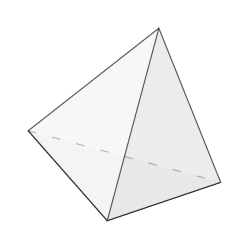
\begin{tikzpicture}
		\coordinate (pic) at (0,0);
		\begin{scope}[shift=(pic), scale=0.8, rotate=-15]
			\coordinate (T) at (pic);
			\coordinate (A) at (-4.5em, -6em);
			\coordinate (B) at (4.5em, -6em);
			\coordinate (C) at (0, -9em);
		\end{scope}
		\draw[fill=gray!10, opacity=0.6] (A) -- (C) -- (B);	% Sisi bawah
		\draw[loosely dashed, opacity=0.6] (A) -- (B);
		\draw[fill=gray!10, opacity=0.6] (T) -- (A) -- (C);	% Sisi kiri
		\draw[fill=gray!25, opacity=0.6] (T) -- (B) -- (C) --cycle;	% Sisi kanan
	\end{tikzpicture} \qquad 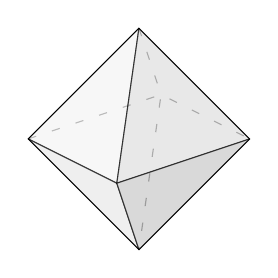
\begin{tikzpicture}
		\coordinate (pic) at (0,0);
		\begin{scope}[shift=(pic), scale=0.8]
			\coordinate (A1) at (pic);
			\coordinate (A2) at (6em, 2em);
			\coordinate (A3) at (10em, 0);
			\coordinate (A4) at (4em, -2em);
			\coordinate (B1) at (5em, 5em);
			\coordinate (B2) at (5em, -5em);
		\end{scope}
		
		\begin{scope}[loosely dashed, opacity=0.6]
			\draw (A1) -- (A2) -- (A3);
			\draw (B1) -- (A2) -- (B2);
		\end{scope}
		\draw[fill=gray!10,opacity=0.6] (A1) -- (A4) -- (B1);
		\draw[fill=gray!20,opacity=0.6] (A1) -- (A4) -- (B2);
		\draw[fill=gray!30,opacity=0.6] (A3) -- (A4) -- (B1);
		\draw[fill=gray!50,opacity=0.6] (A3) -- (A4) -- (B2);
		\draw (B1) -- (A1) -- (B2) -- (A3) --cycle;
	\end{tikzpicture}\end{center}
	dan sebagainya. Dua polihedron disebut kongruen jika keduanya dapat ditumpangtindihkan melalui serangkaian translasi, pencerminan, dan rotasi. Selanjutnya, kita meninjau polihedron hanya hingga kekongruenan. Definisi yang ketat termasuk dalam analisis konveks.
	
	Jika dua polihedron $P, P'$ masing-masing dapat dipotong menjadi banyaknya bagian polihedron kecil yang sama (misalnya dengan pemotongan oleh bidang)
	\[ P = P_1 \cup \ldots \cup P_r, \quad P' = P'_1 \cup \cdots \cup P'_r \]
	sehingga setiap $P_i$ kongruen dengan $P'_i$, maka $P$ dan $P'$ disebut \emph{kongruen-pembedahan}. Sewajarnya, setiap konsep volume polihedron yang masuk akal harus invarian terhadap kongruensi-pembedahan; definisi yang bersesuaian juga tersedia dalam ruang dua dimensi $\mathbb{E}^2$. Untuk mempelajari volume polihedron, Euklides menggunakan apa yang disebut metode penghabisan Eudoksos dalam Buku XI \emph{Unsur-unsur}, suatu pendahulu konsep limit modern. Banyak matematikawan, termasuk Gauss, tidak sepenuhnya puas dan bertanya apakah kesamaan volume dua polihedron dapat diputuskan melalui metode pembedahan elementer. Jawabannya afirmatif dalam dua dimensi (Teorema Bolyai--Gerwien; lihat \cite[Theorem 24.7]{Har00}), sedangkan kasus tiga dimensi merupakan salah satu masalah yang diajukan Hilbert pada Kongres Matematikawan Internasional tahun 1900. Berikut garis besar jawaban negatif M.\ Dehn.
		\begin{enumerate}[(i)]
			\item Untuk setiap rusuk $E$ dari polihedron $P$, tuliskan panjangnya sebagai $\ell(E) \in \R$. Sudut dihedralnya $\angle E \in \R/\pi\Z$ didefinisikan sebagai berikut: pilih suatu bidang $L$ yang melalui titik interior $x$ dari $E$ dan tegak lurus terhadap $E$; sudut dalam poligon $L \cap P$ pada verteks $x$ ialah $\angle E$. Definisikan invarian Dehn dari $P$ sebagai
				\[ \delta(P) := \sum_{E: \text{rusuk}} \ell(E) \otimes \angle E \quad \in A. \]
				% Gambar
				Buktikan bahwa $\delta$ untuk setiap kubus adalah $0$. Buktikan bahwa $\delta$ untuk suatu tetrahedron beraturan dengan panjang rusuk $\ell$ adalah $6\ell \otimes \arccos(\frac{1}{3})$.
			\item Buktikan bahwa jika suatu bidang $\alpha=0$ dalam ruang memotong polihedron $P$ menjadi dua bagian $P = P_+ \cup P_-$, dengan $P_{\pm} := P \cap \{\pm\alpha \geq 0 \}$, maka $\delta(P) = \delta(P_+) + \delta(P_-)$. Dengan demikian, invarian Dehn dipertahankan oleh kongruensi-pembedahan.
				\begin{hint}
					Tinjau rusuk-rusuk baru yang dihasilkan oleh irisan bidang $\alpha=0$; keadaan tipikal mencakup yang berikut.
					\begin{center}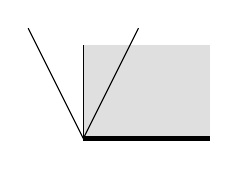
\begin{tikzpicture}[scale=0.7]
						\fill[gray!25] (0,0) rectangle (2.3, 1.7);
						\draw (0,0) -- (-1,2); \draw (0,0) -- (1,2); \draw[ultra thick] (0,0) -- (2.3, 0);
						\draw (0,0) -- (0,1.7);
					\end{tikzpicture} \qquad 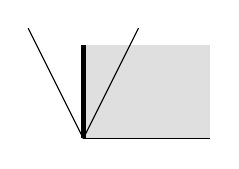
\begin{tikzpicture}[scale=0.7]
						\fill[gray!25] (0,0) rectangle (2.3, 1.7);
						\draw (0,0) -- (-1,2); \draw (0,0) -- (1,2); \draw (0,0) -- (2.3, 0);
						\draw[ultra thick] (0,0) -- (0,1.7);
					\end{tikzpicture} \\ \vspace{2em}
					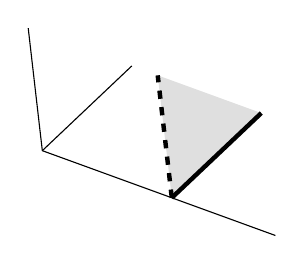
\begin{tikzpicture}[scale=0.7, rotate=-20]
						\fill[gray!25] (0,0) -- (1,2) -- (-1,2) --cycle;
						\draw (-2.5, 0) -- (2, 0);
						\draw[ultra thick] (0,0) -- (1,2); \draw[dashed, ultra thick] (0,0) -- (-1,2);
						\draw (-2.5,0) -- (-3.5, 2); \draw (-2.5,0) -- (-1.5, 2);
					\end{tikzpicture} \qquad 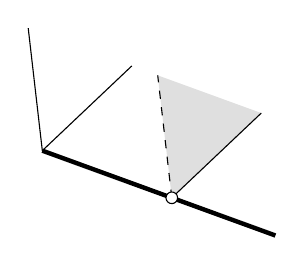
\begin{tikzpicture}[scale=0.7, rotate=-20]
						\fill[gray!25] (0,0) -- (1,2) -- (-1,2) --cycle;
						\draw (0,0) -- (1,2); \draw[dashed] (0,0) -- (-1,2);
						\draw[ultra thick] (0,0) -- (-2.5,0); \draw[ultra thick] (0,0) -- (2,0);
						\filldraw[fill=white] (0,0) circle[radius=3pt];
						\draw (-2.5,0) -- (-3.5, 2); \draw (-2.5,0) -- (-1.5, 2);
					\end{tikzpicture}\end{center}
					Garis tebal menyatakan rusuk baru yang sedang ditinjau, sedangkan daerah berarsir ialah bagian yang dipotong oleh bidang. Gunakan sifat hasil kali tensor untuk memperoleh $\delta(P) = \delta(P_+) + \delta(P_-)$.
				\end{hint}
			\item Buktikan bahwa suatu tetrahedron beraturan tidak mungkin kongruen-pembedahan dengan sebuah kubus, walaupun volumenya dapat sama. \hint{Masalah ini tereduksi menjadi $\arccos(\frac{1}{3}) \notin \Q\pi$. Pembaca dapat mencoba memberikan argumen langsung, atau menerima Proposisi \ref{prop:cos-rationality} yang akan dibuktikan kemudian.}
		\end{enumerate}
		Catatan: J.-P.\ Sydler (1965) membuktikan bahwa dua polihedron $P, P'$ dalam $\mathbb{E}^3$ kongruen-pembedahan jika dan hanya jika keduanya mempunyai volume dan invarian Dehn yang sama.
	\item Buktikan bahwa konstruksi $A \mapsto A^\vee$ dalam Korolari \ref{prop:finite-duality} memberikan suatu ekuivalensi dari kategori grup abelian berhingga $\cate{FinAb}$ ke $\cate{FinAb}^\text{op}$, dan tunjukkan bahwa konstruksi tersebut merupakan fungtor eksak.
	\item Untuk suatu grup abelian bereksponen $A$, buktikan bahwa homomorfisme $\iota_A$ dalam \eqref{eqn:ab-group-duality} bersifat injektif.
		\begin{hint} Kasus grup siklik mudah ditangani. Gunakan sifat bahwa $\Q/\Z$ merupakan modul $\Z$ yang dapat dibagi untuk beralih ke kasus umum. \end{hint}
	\item Lengkapi pembuktian Proposisi \ref{prop:5-lemma-mod} dengan pengejaran diagram.
\end{Exercises}
